\documentclass[a4paper, 12pt]{report}

\usepackage[utf8]{inputenc}
\usepackage{graphicx} 
\usepackage{makecell}
\usepackage{float}
\usepackage[nottoc]{tocbibind}
\usepackage{titlesec}
\usepackage[strings]{underscore}

\titleformat{\chapter}[display]
    {\normalfont\huge\bfseries}{\chaptertitlename\ \thechapter}{20pt}{\Huge}
\titlespacing*{\chapter}{0pt}{0pt}{5pt}

\graphicspath{{figures/}}
% Title Page
\title{\textbf{eHealth Documentation}\\Java - Objected Oriented Programming}
\author{Johannes Jobst\\Marin-Petru Hincu\\Pascal Kautzmann\\Hania Anjum Chatha}


\begin{document}
\maketitle


\tableofcontents
\listoffigures

\chapter{Introduction}
{\tiny (Johannes Jobst, 1300563)\\}
This documentation is about our results of creating a smart eHealth consulting system by using the objected oriented programming language Java. We give an overview how our application is structured, how we proceeded the project, how the tasks were distributed in the team and much more.
\\
\\
\\

{\let\clearpage\relax \chapter{Project motivation}}
{\tiny (Marin-Petru Hincu, 1268171)\\}
This chapter will present some aspects that motivated us as a team, but also individually, to work on the eHealth project.
One important aspect was exploring the possibilities we had to work on the same project simultaneously. It was going to be our first experience working on a project with specific requirements as a small group, so we were very excited. \\
The other important aspect was learning more about the topics we needed to study in order to successfully finish the project. Some topics we were most interested in will be discussed in the following.\\
Creating an Application which uses a database to store most of its user information was one interesting topic. We knew that most applications nowadays heavily use databases, but we did not know how it is implemented. Learning more about how the application can be connected to the database and successfully implementing some of the relations between the application and the database was a very rewarding experience. \\
Knowing we would learn more about the practical implementation of distance calculations between addresses was also a motivation. Most of us use these tools on a daily basis, either by looking up an address on Google Maps or by searching for a restaurant on your favourite delivery app. However, most of us do not know how those features are implemented into our applications, so we were very excited about implementing those features ourselves.
A final topic which we were motivated to learn more about was encryption. The basics of encryption were common knowledge for all group members. Nevertheless, none of us had experience in implementing encryption algorithms for storing encrypted passwords in a database. Security is a very important aspect in the world of software, so we were eager to learn more about the practical implementation methods. \\
These were some aspects which gave us a great amount of motivation at the beginning and during the project. In general, we were motivated to learn more about the above mentioned topics, because we knew that the accumulated experiences during the project would make us better software developers.
\\
\\
\\

{\let\clearpage\relax \chapter{Project description}}
{\tiny (Johannes Jobst, 1300563)\\}
Our eHealth application is designed that a user doesn't anymore need to call a doctor via the telephone if he or she has a health problem. \\
Instead it provides a whole new experience for people to creating an appointment. They now are able to create an account in our eHealth application. With this account they can login into the system and specify their health problem. The smart application then displays, based on the symptoms you have and the distance radius in which a doctor should be, all suggested doctors for you. In the next step the user is able to make an appointment at one of these doctors. \\
Furthermore our eHealth application displays for logged in users all upcoming appointments they have. Adding to that the user has the ability to edit or delete a certain appointment. \\ In the following Figure 3.1 you can see a brief overview of the main window of our eHealth application.
\\
Because our user storing is implemented in a database [2] our eHealth application has an additional admin account which is available with special login data. In this admin view the admin is able to manage the users like edit personal information of them but also deleting them.
\\
\begin{figure}[!h]
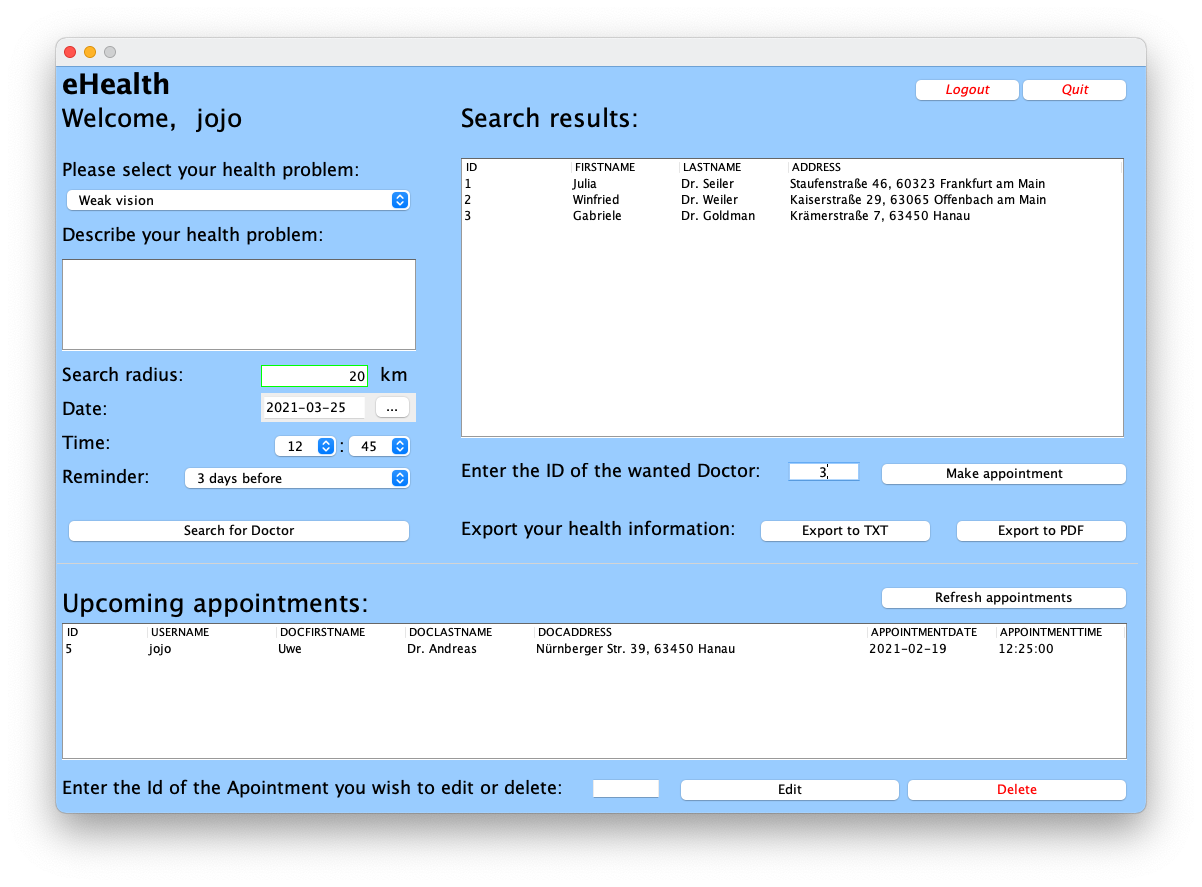
\includegraphics[width=\linewidth]{main.png} 
\caption{eHealth main window under MacOS}
\end{figure}

\chapter{Team organization}
\section{Meetings}
{\tiny (Johannes Jobst, 1300563)\\}
At the beginning of the project we first of all thought it would be very useful 
to have a fixed day in the week to have a meeting about our project. \\
In our weekly meetings we discussed how to do and implement certain tasks in the project.
At the end of every meeting we came to a task distribution and defined who is
responsible for which task. 

\section{Task distribution}
Johannes Jobst was responsible for everything concerning the Graphical User Interface.
He also implemented the most parts of ERROR handling. For example the check whether the given
input by the user was correct. But also checks that appointments could not be made in the past. \\ \\
Marin-Petru Hincu designed the database, created the necessary tables and embedded the database into the project [1]. He provided methods for connecting to the database, manipulating, and retrieving data from the database. Marin did also implement the user class and its functionality. \\ \\
Pascal Kautzmann was responsible for implementing the e-mail function, the password hashing, the reminder function and the usability of the OpensStreetMaps-API \\ 
	\\
Hania Anjum Chatha was responsible for deciding the health problems of patients and names, addresses of the doctor. She also tried to make database tables for appointment and doctor.

\section{Development timeline}
{\tiny (Johannes Jobst, 1300563)\\}
At the beginning we started to create a GitHub repository for our project. We then constructed a basic GUI construct for the login window. With this basic construct we already were able to implement our database in the project. \\
After implementing the database we were already able to create new accounts and add them to it. As a result the login with existing accounts to our system already worked. \\
In the next step we added password encryption to the login data. \\
We then thought that a convert of our project to a Maven project would be very handy, because we needed to implement some "Plugins" like the H2 Database [2] or the JDatePicker [5] to our Java project.
\\
After that we build the admin window and add step by step the full functionality to the GUI of the admin. We created a table to display all users in the database. Made buttons to edit a user via the "editUserWindow" or delete a user.
\\
After finishing with the admin window we focused more on the main part of the application. Therefore it was required to implement a 2 factor authentication. We implemented that with a new window.
\\
As a next step we started to develop all functionalities for the main window. We added all necessary GUI elements and connected them to the database. We implemented a "editAppointment" window to shift upcoming appointments. Concomitant with that we finally implemented the reminder functionality and also the health information export function.
\\
So finally our program is finished. At the end we had only to fix some bugs where something was not probably working. 

\section{Tools}
{\tiny (Johannes Jobst, 1300563)\\}
For our project the whole team used the Eclipse IDE, because of some small differences in other IDEs. In Eclipse itself we used the WindowBuilder to design our GUI.\\
Our main tool for working on the project as a team was GitHub. There we have a central repository for storing all project data like the complete source code but also the project documentation. It makes the working on the project very comfortable and easy because of the ability to work simultaneously on the code.

%All contributors to the project linked their functionality to the respective part of the UI%


\chapter{Technical description}
\section{Requirements}
\subsection{Overview}
{\tiny (Marin-Petru Hincu, 1268171)\\}
The following figure represents all components needed for the project and their correlation.
\begin{figure}[!h]
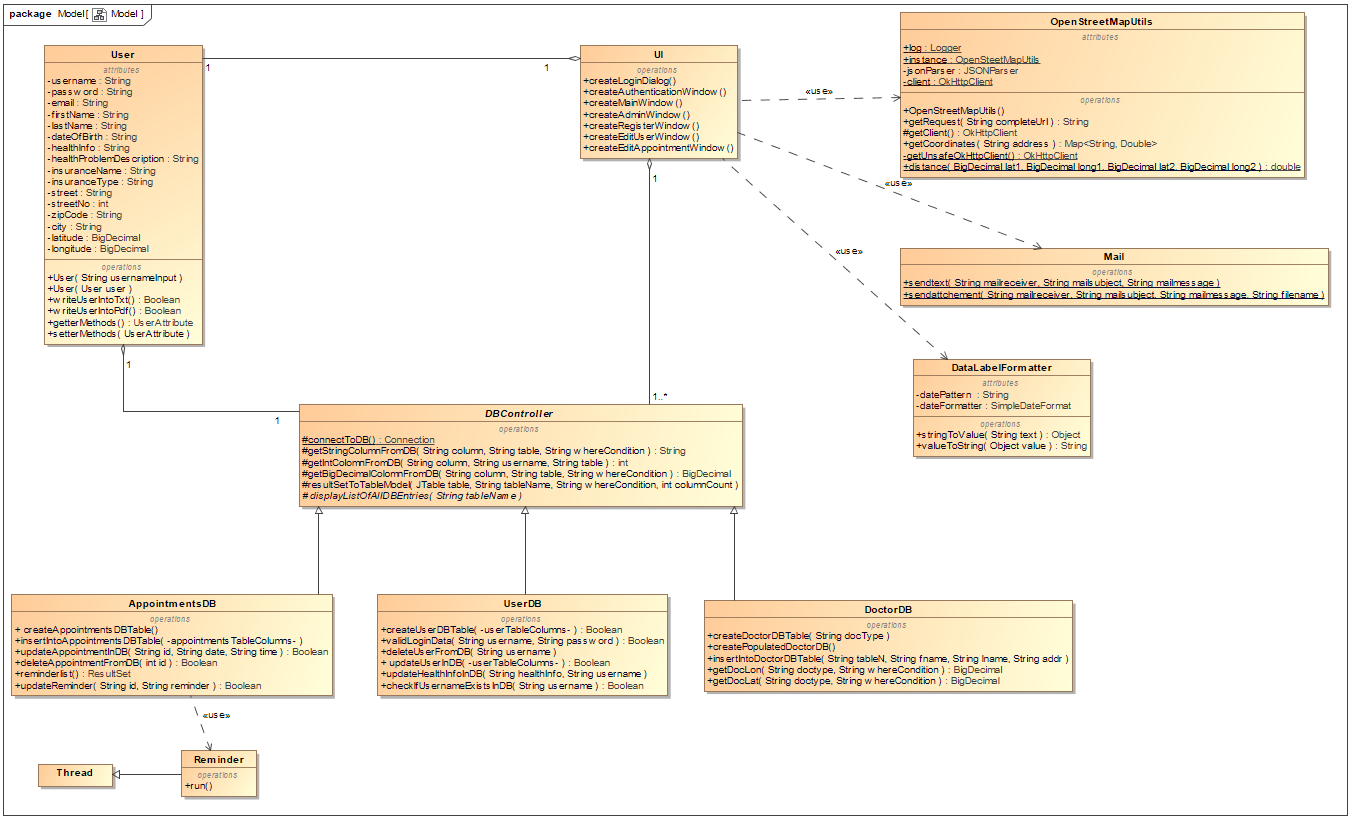
\includegraphics[width=\linewidth]{clImg.png} 
\caption{Class diagram for the eHealth project}
\end{figure}
\\The user class represents the user of the eHealth application. Every piece of data needed for the user is stored as an attribute. Some methods allow for modifications and obtaining information about the user. Methods for writing user information into an txt or pdf are also available. \\
DBController contains important methods for connecting to the database modifying its contents and retrieving data. The classes AppointmentsDB, UserDB and DoctorDB are derived from the DBController and are used for creating and querying the respective database tables. The AppointmentsDB also uses the class reminder which allows threading the appointments table.\\The class named UI represents all User Interfaces used in the project. Some graphical user interfaces make use of the class OpenStreetMapUtils, which provides useful functionality for determining the location of a user or a doctor and calculating the distance between both. The class Mail is also used for sending out E-mails whenever this is necessary in the project. Finally, the class DateLabelFormatter is used by the UI to ensure correctly formatted dates for the appointments. \\
As illustrated in Figure 5.1, each user contains one DBController and the UI contains one User and multiple instances of the DBController. The reason being that in some cases the UI needs to have access to all three database tables.\\ The following pages will go in more detail about the components of the UI and their interactions.

\subsection{Activity overview}
{\tiny (Johannes Jobst, 1300563)\\}
In Figure 5.2 you can see how the activity flow of our program works.\\
First of all our program displays an login window where you have the choice to create a new account or to login with your account into our eHealth system. If you type in your username and your password correctly the system will check the authentication via 2 factor authentication, so it sends you a mail with a random code which you must type in the dialog. After validation the system checks whether you are an admin or a user.\\
In the admin view the admin has the ability to show up all registered users and can edit their personal data or delete them.
In the user view the user has the ability to make appointments after selecting his health problem and providing some more data. The system then searches for matching doctors and displays them. Now the user can choose his doctor out of the results and make an appointment.\\
Additionally the user can display the upcoming appointments and make changes of the date and the time or even delete the appointment.
The last main functionality he has is that he can export his health information either in pdf or txt format.


\begin{figure}[!h]
	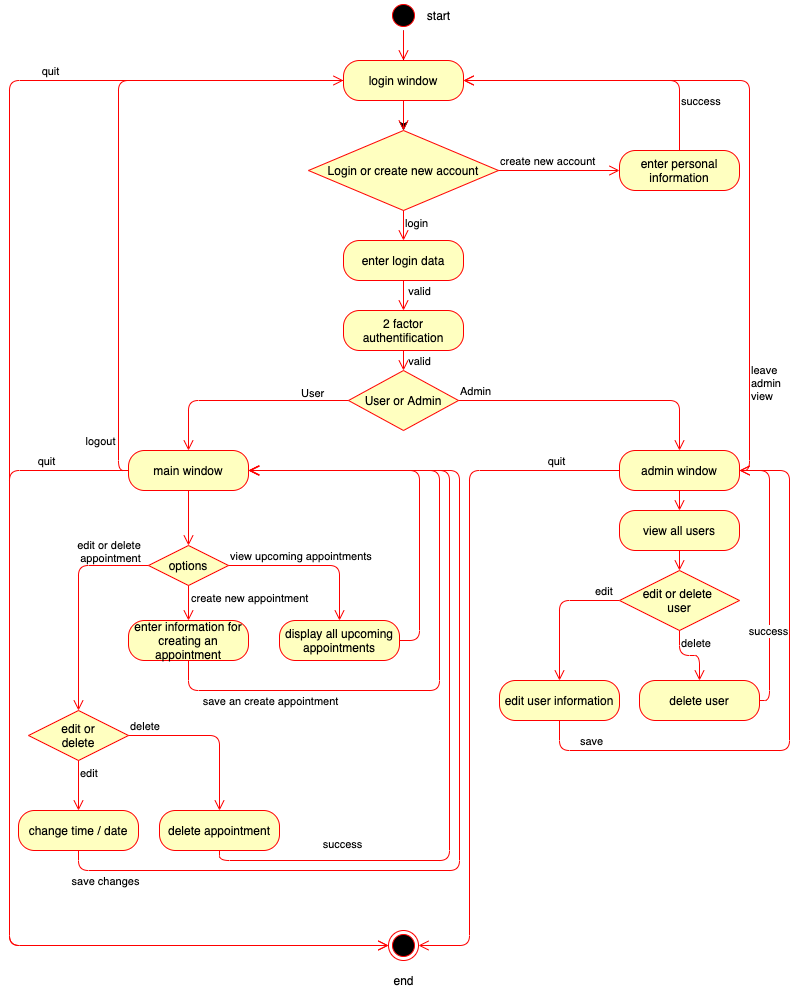
\includegraphics[width=\linewidth]{eHealth_Activity.png}
	\caption{Activity diagram for the eHealth project}
\end{figure}

\subsection{Account creation}
{\tiny (Johannes Jobst, 1300563)\\}
The first main requirement of our program is the account creation.\\
If the User uses the application for the first time he has the ability to create a new eHealth account. Therefore he has to enter his firstname, lastname, email address, address information, date of birth, insurance type and his insurance name.
If the user confirms, the entered data is checked for correctness.
The Validation of the email address happens by checking if the email has the right format (eg. max@mustermann.de) [6]. For validating the address we use the API of OpenStreetMaps and check if the given address exists.
The username must be unique in our database, so the system checks whether its already existing. For the insurance type one of the given types must be selected.
For the rest of the Fields the system checks that they aren't empty and not longer than the capacity of the corresponding field in the database.
With this error handling we ensure that ours system doesn't run into database errors.\\
If every information is typed in correctly the account is now created.
%\begin{figure}[!h]
%\includegraphics[width=\linewidth]{login_Activity.png} 
%\caption{Class diagram for the eHealth project}
%\end{figure}
\subsection{Login}
{\tiny (Johannes Jobst, 1300563)\\}
If the user already has an account he is able to login with his username and password. In the next step there is a database comparison and when the data is valid there appears a 2 factor authentication window. In this window the user is asked to enter the code which is send to him via email. This ensures that no unauthorised person can log in even with knowing the login data. All in all this ensures that the very sensitive health and user information is kept secure.

\subsection{Password}
{\tiny ( Pascal Kautzmann, 1320404)\\}
The password is saved as a hash, because it is really difficult and time-consuming to recreate a hashed string.
The password is hashed with the from javax.crypto provided functions. It uses a SHA512 algorithm to hash, the password is also "Salted", so that if two users have the same password, the hashed password is still different.

\subsection{E-Mail}
{\tiny (Pascal Kautzmann, 1320404)\\}
To send e-mails the javax.mail classes are used. An e-mail address to send an e-mail is predefined, and can't be changed by the user,
because mail services, like g-mail, don't allow unverified apps as long as  less secure app access is deactivated. [7]


\subsection{Admin view}
{\tiny (Johannes Jobst, 1300563)\\}
If the user enters admin login data into login dialog the system will open an admin view. The admin there has the ability to view all users. This is implemented via an SQL query out of the user table in the database. The admin has also the option to edit the personal informations of users. Therefore a looking almost like the register window pops up, where he is able to make changes.
With the same error handling like in the account creation the system is prevented from any errors.


\subsection{Searching for a doctor}
{\tiny (Pascal Kautzmann, 1320404)\\}
In the main window the user has the possibility to search for a doctor, for that the user has to provide some data.
\begin{figure}[!h]
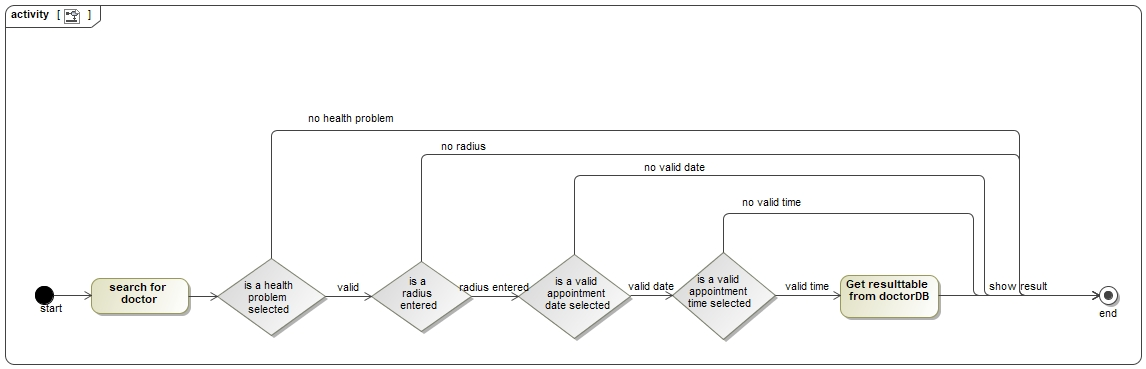
\includegraphics[width=\linewidth]{doctorsearch.jpg} 
\caption{Activity diagram for searching a doctor}
\end{figure}
\\First the user needs to select his or her health problem with the help of a drop-down list, where we predefined some health problems.
Then the user has the possibility to better describe their problem and give some more information.
Next they have to select the search radius, so it is possible only to search for a doctor in the given radius around their address.
Now the user can select the date and time when he or she wants to have an appointment.
The last information needed is whether they want to receive a reminder and if yes how long before the appointment.
If the user presses the button "Search for Doctor" the program first checks if all necessary data is given and in a correct format. Then it gets the list of possible doctors from the Doctor-Database and displays them, so that the user can select one.


\subsection{Creating an Appointment}
{\tiny (Hania Anjum Chatha, 1293609)\\}
In figure [5.4] we add multiple features to make the appointment easily for patients. After logging in into the system, they can make and cancel their appointment. For making appointment, patients can select the department and according to that department they can select a doctor and their preferred time. For canceling the appointment, patients are required to select the registered appointment and click on the cancel button.

\begin{figure}[!h]
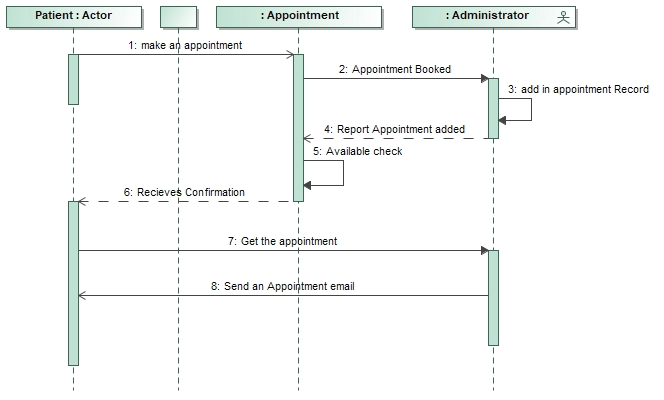
\includegraphics[width=\linewidth]{sequence_appointments.png}
\caption{Sequence diagram for creating an appointment}
\end{figure}

\subsection{Editing an Appointment}
{\tiny (Marin-Petru Hincu, 1268171)\\}
In the main window the user has the possibility to view the appointments he made. He can also edit or delete these appointments.
\begin{figure}[!h]
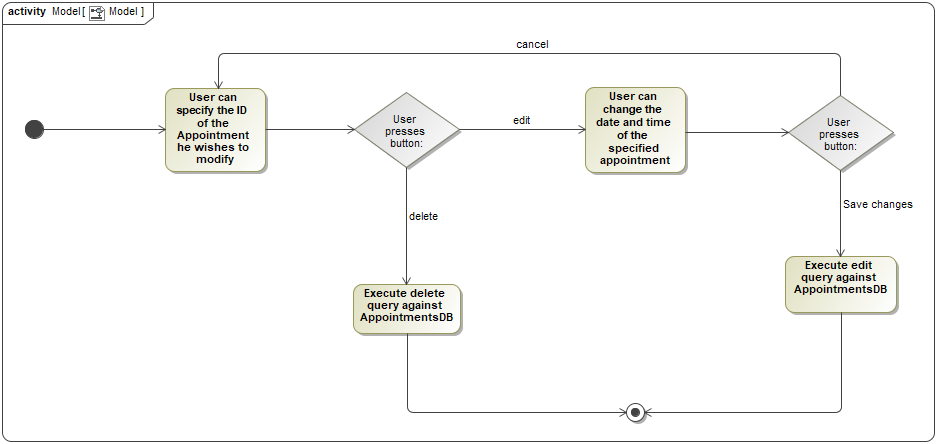
\includegraphics[width=\linewidth]{acImg.png} 
\caption{Activity diagram for deleting and editing an appointment}
\end{figure}
\\In the appointments table displayed in the main window, the user has to select the id of the appointment he wishes to edit or delete. After the user pasted in the id into the respective text field, he can either press the button "delete" or "edit". If the user presses "delete", he must first confirm the action and then the selected appointment is deleted from the table. If the user presses "edit", he gets redirected to a new window, where he can then change the date and time of the appointment. The user must then press "save" for the changes to be saved in the appointments table, and he returns to the main window. However, if the user presses "cancel", he returns to the main window without modifying anything.


\subsection{Reminder}
{\tiny (Pascal Kautzmann, 1320404)\\}
The reminder runs in a separate thread, so it doesn't interfere with the rest of the program.
The reminder will check every minute whether there is an entry in the Appointment-database that requires a reminder. 
Then it sends to the user who wants the reminder an e-mail with the appointment details.

\subsection{Exporting health information}
{\tiny (Marin-Petru Hincu, 1268171)\\}
By pressing the button "Export health info to TXT/PDF", located in the main window, the health information stored about the user can be exported as a text file or as a pdf [3].\\ The file is by default exported to the desktop of the user.

\chapter{Challenges}
\subsection{Implementing the database}
{\tiny (Marin-Petru Hincu, 1268171)\\}
The first and very challenging step in the project was implementing the database. It was difficult at first, because we were completely new to that subject and had to do a lot of research before even beginning with the implementation [4]. We then decided to use an embedded version of the H2 database [2].
Using an embedded database, it wasn't necessary for each of us to have a local database running. Another advantage is the high portability and increased performance this concept provides.\\
Now having the database all set up, it was important to create the corresponding database tables as precise as possible, knowing that those tables are the basis for the whole application. \\

\subsection{JDatePicker}
{\tiny (Johannes Jobst, 1300563)\\}
When we first started our project we implemented every date user input using a normal JTextfield. But after a while we run into problems with error handing with wrong dates. We then though of the implementation via a JDatePicker [5]. This made the error handling easy because you can no more enter a wrong date format. You only can choose a date out of the calendar.

\subsection{Password-Encryption}
{\tiny (Pascal Kautzmann, 1320404)\\}
Another challenge was to find out how passwords can be stored securely in a database, so we had to research. We found out passwords are stored in hash, "Hashing is the process of generating a string, or hash, from a given message using a mathematical function known as a cryptographic hash function" [8], so if someone sees the database he can't know the original password. \\
There are a some implementations in java for hashing, like MD5 and SHA-512, but these are old and weak algorithms, so we decided to use the PBKDF2 function. To ensure that even if two users have the same password we still have different hashes in the database we needed to use a salt for the password.


\subsection{Distance of search}
{\tiny (Pascal Kautzmann, 1320404)\\}
We now had to find out how to calculate the distance of search, we found out that it's easy to calculate a distance between the coordinates, but now we didn't know how we could get the coordinate of a given address. After a search we found two options, Google-Maps and OpenStreetMap, booth have an option to use them with java, but OpenStreetMap has the advantage
that it doesn't need an account, to enable the api, like google. "OpenStreetAPI provides GET request support, with open to get the data in json." [9]\\
With this implementation we can store the coordinates from the given address, now we only needed a simple distance calculation [10]. 
 

\chapter{Conclusion}
{\tiny (Hania Anjum Chatha, 1293609)\\}
In Conclusion, our smart E-health Consulting System simplifies the management process by providing fast services with high accuracy and security. Minimising human effort and is needed and it  makes an efficient and accessible patient record. Using system analysis and design techniques like class diagrams, sequence diagrams, and activity diagrams helped us to design an error free system. The Smart E-health Consulting system accommodates scalability, allowing flexibility within the system to edit or delete patient records and arrange quick doctor appointments without problems. \\
In this project we maintain the patient and doctor data, where patients can register their appointment. Overall, this projects' aim is to manage the appointment, patients and doctor details. The Smart E-health Consulting System technology is a future-oriented good alternative for our patients and doctors.

\chapter{Sources}

[1] Oracle, The Java™ Tutorials, Using JDBC with GUI API,\\
https://docs.oracle.com/javase/tutorial/jdbc/basics/		jdbcswing.html, \\22.01.2021 17:10 \\\relax
[2] Thomas Mueller, H2 Features, https://www.h2database.com/html/features.html,\\ 11.02.2021 13:35 \\\relax
[3] Baeldung, Creating PDF Files in Java, \\https://www.baeldung.com/java-pdf-creation, 06.02.2021 19:15 \\\relax
[4] Tutorialspoint, H2 Database - JDBC Connection, \\https://www.tutorialspoint.com/h2_database/index.htm, 16.12.2020 21:55 \\\relax
%author, publication date, page title, site title, URL, date accessed
[5] Ashane Alvis, Wie implementiere ich JDatePicker?, \\https://www.javaer101.com/de/article/1525991.html, 24.01.2021 17:30 \\\relax
[6] Aaron Davidson, What is the best Java email address validation method?, \\https://stackoverflow.com/questions/624581/what-is-the-best-java-email-address-validation-method, \\10.01.2021 20:45 \\\relax
[7]Google, Mit der Mail API E-Mails senden, \\https://cloud.google.com/appengine/docs/standard/java/mail/sending-mail-with-mail-api?hl=de, 12.10.2020\\\relax
[8]Sam Millington,Hashing a Password in Java,\\https://www.baeldung.com/java-password-hashing, 09.01.2021 \\\relax
[9]Muasir Khalil, Geo data Leveraging OpenStreetMap,\\https://medium.com/@muasir_33255/geo-data-leveraging-openstreetmap-11a5fe2cf9dc, 03.07.2020\\\relax
[10]Martin Kompf, Distance calculation,\\https://www.mkompf.com/gps/distcalc.html, 2019


\end{document}